\upaper{15}{The Seven Superuniverses}
\uminitoc{The Superuniverse Space Level}
\uminitoc{Organization of the Superuniverses}
\uminitoc{The Superuniverse of Orvonton}
\uminitoc{Nebulae --- The Ancestors of Universes}
\uminitoc{The Origin of Space Bodies}
\uminitoc{The Spheres of Space}
\uminitoc{The Architectural Spheres}
\uminitoc{Energy Control and Regulation}
\uminitoc{Circuits of the Superuniverses}
\uminitoc{Rulers of the Superuniverses}
\uminitoc{The Deliberative Assembly}
\uminitoc{The Supreme Tribunals}
\uminitoc{The Sector Governments}
\uminitoc{Purposes of the Seven Superuniverses}
\author{Universal Censor}
\vs p015 0:1 As far as the Universal Father is concerned --- as a Father --- the universes are virtually nonexistent; he deals with personalities; he is the Father of personalities. As far as the Eternal Son and the Infinite Spirit are concerned --- as creator partners --- the universes are localized and individual under the joint rule of the Creator Sons and the Creative Spirits. As far as the Paradise Trinity is concerned, outside Havona there are just seven inhabited universes, the seven superuniverses which hold jurisdiction over the circle of the first post\hyp{}Havona space level. The Seven Master Spirits radiate their influence out from the central Isle, thus constituting the vast creation one gigantic wheel, the hub being the eternal Isle of Paradise, the seven spokes the radiations of the Seven Master Spirits, the rim the outer regions of the grand universe.
\vs p015 0:2 Early in the materialization of the universal creation the sevenfold scheme of the superuniverse organization and government was formulated. The first post\hyp{}Havona creation was divided into seven stupendous segments, and the headquarters worlds of these superuniverse governments were designed and constructed. The present scheme of administration has existed from near eternity, and the rulers of these seven superuniverses are rightly called Ancients of Days.
\vs p015 0:3 Of the vast body of knowledge concerning the superuniverses, I can hope to tell you little, but there is operative throughout these realms a technique of intelligent control for both physical and spiritual forces, and the universal gravity presences there function in majestic power and perfect harmony. It is important first to gain an adequate idea of the physical constitution and material organization of the superuniverse domains, for then you will be the better prepared to grasp the significance of the marvellous organization provided for their spiritual government and for the intellectual advancement of the will creatures who dwell on the myriads of inhabited planets scattered hither and yon throughout these seven superuniverses.
\usection{The Superuniverse Space Level}
\vs p015 1:1 Within the limited range of the records, observations, and memories of the generations of a million or a billion of your short years, to all practical intents and purposes, Urantia and the universe to which it belongs are experiencing the adventure of one long and uncharted plunge into new space; but according to the records of Uversa, in accordance with older observations, in harmony with the more extensive experience and calculations of our order, and as a result of conclusions based on these and other findings, we know that the universes are engaged in an orderly, well\hyp{}understood, and perfectly controlled processional, swinging in majestic grandeur around the First Great Source and Centre and his residential universe.
\vs p015 1:2 We have long since discovered that the seven superuniverses traverse a great ellipse, a gigantic and elongated circle. Your solar system and other worlds of time are not plunging headlong, without chart and compass, into unmapped space. The local universe to which your system belongs is pursuing a definite and well\hyp{}understood counterclockwise course around the vast swing that encircles the central universe. This cosmic path is well charted and is just as thoroughly known to the superuniverse star observers as the orbits of the planets constituting your solar system are known to Urantia astronomers.
\vs p015 1:3 Urantia is situated in a local universe and a superuniverse not fully organized, and your local universe is in immediate proximity to numerous partially completed physical creations. You belong to one of the relatively recent universes. But you are not, today, plunging on wildly into uncharted space nor swinging out blindly into unknown regions. You are following the orderly and predetermined path of the superuniverse space level. You are now passing through the very same space that your planetary system, or its predecessors, traversed ages ago; and some day in the remote future your system, or its successors, will again traverse the identical space through which you are now so swiftly plunging.
\vs p015 1:4 \pc In this age and as direction is regarded on Urantia, superuniverse number one swings almost due north, approximately opposite, in an easterly direction, to the Paradise residence of the Great Sources and Centres and the central universe of Havona. This position, with the corresponding one to the west, represents the nearest physical approach of the spheres of time to the eternal Isle. Superuniverse number two is in the north, preparing for the westward swing, while number three now holds the northernmost segment of the great space path, having already turned into the bend leading to the southerly plunge. Number four is on the comparatively straightaway southerly flight, the advance regions now approaching opposition to the Great Centres. Number five has about left its position opposite the Centre of Centres while continuing on the direct southerly course just preceding the eastward swing; number six occupies most of the southern curve, the segment from which your superuniverse has nearly passed.
\vs p015 1:5 Your local universe of Nebadon belongs to Orvonton, the seventh superuniverse, which swings on between superuniverses one and six, having not long since (as we reckon time) turned the south\hyp{}eastern bend of the superuniverse space level. Today, the solar system to which Urantia belongs is a few billion years past the swing around the southern curvature so that you are just now advancing beyond the south\hyp{}eastern bend and are moving swiftly through the long and comparatively straightaway northern path. For untold ages Orvonton will pursue this almost direct northerly course.
\vs p015 1:6 Urantia belongs to a system which is well out towards the borderland of your local universe; and your local universe is at present traversing the periphery of Orvonton. Beyond you there are still others, but you are far removed in space from those physical systems which swing around the great circle in comparative proximity to the Great Source and Centre.
\usection{Organization of the Superuniverses}
\vs p015 2:1 Only the Universal Father knows the location and actual number of inhabited worlds in space; he calls them all by name and number. I can give only the approximate number of inhabited or inhabitable planets, for some local universes have more worlds suitable for intelligent life than others. Nor have all projected local universes been organized. Therefore the estimates which I offer are solely for the purpose of affording some idea of the immensity of the material creation.
\vs p015 2:2 \pc There are seven superuniverses in the grand universe, and they are constituted approximately as follows:
\vs p015 2:3 \ublistelem{1.}\bibnobreakspace \bibemph{The System.} The basic unit of the supergovernment consists of about 1,000 inhabited or inhabitable worlds. Blazing suns, cold worlds, planets too near the hot suns, and other spheres not suitable for creature habitation are not included in this group. These 1,000 worlds adapted to support life are called a system, but in the younger systems only a comparatively small number of these worlds may be inhabited. Each inhabited planet is presided over by a Planetary Prince, and each local system has an architectural sphere as its headquarters and is ruled by a System Sovereign.
\vs p015 2:4 \ublistelem{2.}\bibnobreakspace \bibemph{The Constellation.} 100 systems (about $10^5$ inhabitable planets) make up a constellation. Each constellation has an architectural headquarters sphere and is presided over by three Vorondadek Sons, the Most Highs. Each constellation also has a Faithful of Days in observation, an ambassador of the Paradise Trinity.
\vs p015 2:5 \ublistelem{3.}\bibnobreakspace \bibemph{The Local Universe.} 100 constellations (about $10^7$ inhabitable planets) constitute a local universe. Each local universe has a magnificent architectural headquarters world and is ruled by one of the co\hyp{}ordinate Creator Sons of God of the order of Michael. Each universe is blessed by the presence of a Union of Days, a representative of the Paradise Trinity.
\vs p015 2:6 \ublistelem{4.}\bibnobreakspace \bibemph{The Minor Sector.} 100 local universes (about $10^9$ inhabitable planets) constitute a minor sector of the superuniverse government; it has a wonderful headquarters world, wherefrom its rulers, the Recents of Days, administer the affairs of the minor sector. There are three Recents of Days, Supreme Trinity Personalities, on each minor sector headquarters.
\vs p015 2:7 \ublistelem{5.}\bibnobreakspace \bibemph{The Major Sector.} 100 minor sectors (about $10^{11}$ inhabitable worlds) make one major sector. Each major sector is provided with a superb headquarters and is presided over by three Perfections of Days, Supreme Trinity Personalities.
\vs p015 2:8 \ublistelem{6.}\bibnobreakspace \bibemph{The Superuniverse.} 10 major sectors (about $10^{12}$ inhabitable planets) constitute a superuniverse. Each superuniverse is provided with an enormous and glorious headquarters world and is ruled by three Ancients of Days.
\vs p015 2:9 \ublistelem{7.}\bibnobreakspace \bibemph{The Grand Universe.} Seven superuniverses make up the present organized grand universe, consisting of approximately seven trillion inhabitable worlds plus the architectural spheres and the one billion inhabited spheres of Havona. The superuniverses are ruled and administered indirectly and reflectively from Paradise by the Seven Master Spirits. The billion worlds of Havona are directly administered by the Eternals of Days, one such Supreme Trinity Personality presiding over each of these perfect spheres.
\vs p015 2:10 \pc Excluding the Paradise\hyp{}Havona spheres, the plan of universe organization provides for the following units:
\vs p015 2:11 Superuniverses\bibdf7
\vs p015 2:12 Major sectors\bibdf70
\vs p015 2:13 Minor sectors\bibdf7,000
\vs p015 2:14 Local universes\bibdf700,000
\vs p015 2:15 Constellations\bibdf70,000,000
\vs p015 2:16 Local systems\bibdf7,000,000,000
\vs p015 2:17 Inhabitable planets\bibdf7,000,000,000,000
\vs p015 2:18 Each of the seven superuniverses is constituted, approximately, as follows:
\vs p015 2:19 One system embraces, approximately\bibdf1,000 worlds
\vs p015 2:20 One constellation (100 systems)\bibdf100,000 worlds
\vs p015 2:21 One universe (100 constellations)\tunemarkup{pgkoboaurahd}{\linebreak}\bibdf10,000,000 worlds
\vs p015 2:22 One minor sector (100 universes)\tunemarkup{pgauraone}{\linebreak}\tunemarkup{pgkoboaurahd}{\linebreak}\bibdf1,000,000,000 worlds
\vs p015 2:23 One major sector (100 minor sectors)\tunemarkup{pgauraone}{\linebreak}\tunemarkup{pgkoboaurahd}{\linebreak}\bibdf100,000,000,000 worlds
\vs p015 2:24 One superuniverse (10 major sectors)\tunemarkup{pgauraone}{\linebreak}\tunemarkup{pgkoboaurahd}{\linebreak}\bibdf1,000,000,000,000 worlds
\vs p015 2:25 \pc All such estimates are approximations at best, for new systems are constantly evolving while other organizations are temporarily passing out of material existence.
\usection{The Superuniverse of Orvonton}
\vs p015 3:1 Practically all of the starry realms visible to the naked eye on Urantia belong to the seventh section of the grand universe, the superuniverse of Orvonton. The vast Milky Way starry system represents the central nucleus of Orvonton, being largely beyond the borders of your local universe. This great aggregation of suns, dark islands of space, double stars, globular clusters, star clouds, spiral and other nebulae, together with myriads of individual planets, forms a watchlike, elongated\hyp{}circular grouping of about \bibfrac{1}{7}\ts{th} of the inhabited evolutionary universes.
\vs p015 3:2 From the astronomical position of Urantia, as you look through the cross section of near\hyp{}by systems to the great Milky Way, you observe that the spheres of Orvonton are travelling in a vast elongated plane, the breadth being far greater than the thickness and the length far greater than the breadth.
\vs p015 3:3 Observation of the so\hyp{}called Milky Way discloses the comparative increase in Orvonton stellar density when the heavens are viewed in one direction, while on either side the density diminishes; the number of stars and other spheres decreases away from the chief plane of our material superuniverse. When the angle of observation is propitious, gazing through the main body of this realm of maximum density, you are looking toward the residential universe and the centre of all things.
\vs p015 3:4 \pc Of the ten major divisions of Orvonton, eight have been roughly identified by Urantian astronomers. The other two are difficult of separate recognition because you are obliged to view these phenomena from the inside. If you could look upon the superuniverse of Orvonton from a position far\hyp{}distant in space, you would immediately recognize the ten major sectors of the seventh galaxy.
\vs p015 3:5 The rotational centre of your minor sector is situated far away in the enormous and dense star cloud of Sagittarius, around which your local universe and its associated creations all move, and from opposite sides of the vast Sagittarius subgalactic system you may observe two great streams of star clouds emerging in stupendous stellar coils.
\vs p015 3:6 The nucleus of the physical system to which your sun and its associated planets belong is the centre of the onetime Andronover nebula. This former spiral nebula was slightly distorted by the gravity disruptions associated with the events which were attendant upon the birth of your solar system, and which were occasioned by the near approach of a large neighbouring nebula. This near collision changed Andronover into a somewhat globular aggregation but did not wholly destroy the two\hyp{}way procession of the suns and their associated physical groups. Your solar system now occupies a fairly central position in one of the arms of this distorted spiral, situated about halfway from the centre out towards the edge of the star stream.
\vs p015 3:7 \pc The Sagittarius sector and all other sectors and divisions of Orvonton are in rotation around Uversa, and some of the confusion of Urantian star observers arises out of the illusions and relative distortions produced by the following multiple revolutionary movements:
\vs p015 3:8 \ublistelem{1.}\bibnobreakspace The revolution of Urantia around its sun.
\vs p015 3:9 \ublistelem{2.}\bibnobreakspace The circuit of your solar system about the nucleus of the former Andronover nebula.
\vs p015 3:10 \ublistelem{3.}\bibnobreakspace The rotation of the Andronover stellar family and the associated clusters about the composite rotation\hyp{}gravity centre of the star cloud of Nebadon.
\vs p015 3:11 \ublistelem{4.}\bibnobreakspace The swing of the local star cloud of Nebadon and its associated creations around the Sagittarius centre of their minor sector.
\vs p015 3:12 \ublistelem{5.}\bibnobreakspace The rotation of 100 minor sectors, including Sagittarius, about their major sector.
\vs p015 3:13 \ublistelem{6.}\bibnobreakspace The whirl of 10 major sectors, the so\hyp{}called star drifts, about the Uversa headquarters of Orvonton.
\vs p015 3:14 \ublistelem{7.}\bibnobreakspace The movement of Orvonton and 6 associated superuniverses around Paradise and Havona, the counterclockwise processional of the superuniverse space level.
\vs p015 3:15 \pc These multiple motions are of several orders: The space paths of your planet and your solar system are genetic, inherent in origin. The absolute counterclockwise motion of Orvonton is also genetic, inherent in the architectural plans of the master universe. But the intervening motions are of composite origin, being derived in part from the constitutive segmentation of matter\hyp{}energy into the superuniverses and in part produced by the intelligent and purposeful action of the Paradise force organizers.
\vs p015 3:16 \pc The local universes are in closer proximity as they approach Havona; the circuits are greater in number, and there is increased superimposition, layer upon layer. But farther out from the eternal centre there are fewer and fewer systems, layers, circuits, and universes.
\usection{Nebulae --- The Ancestors of Universes}
\vs p015 4:1 While creation and universe organization remain forever under the control of the infinite Creators and their associates, the whole phenomenon proceeds in accordance with an ordained technique and in conformity to the gravity laws of force, energy, and matter. But there is something of mystery associated with the universal force\hyp{}charge of space; we quite understand the organization of the material creations from the ultimatonic stage forward, but we do not fully comprehend the cosmic ancestry of the ultimatons. We are confident that these ancestral forces have a Paradise origin because they forever swing through pervaded space in the exact gigantic outlines of Paradise. Though nonresponsive to Paradise gravity, this force\hyp{}charge of space, the ancestor of all materialization, does always respond to the presence of nether Paradise, being apparently circuited in and out of the nether Paradise centre.
\vs p015 4:2 The Paradise force organizers transmute space potency into primordial force and evolve this prematerial potential into the primary and secondary energy manifestations of physical reality. When this energy attains gravity\hyp{}responding levels, the power directors and their associates of the superuniverse regime appear upon the scene and begin their never\hyp{}ending manipulations designed to establish the manifold power circuits and energy channels of the universes of time and space. Thus does physical matter appear in space, and so is the stage set for the inauguration of universe organization.
\vs p015 4:3 This segmentation of energy is a phenomenon which has never been solved by the physicists of Nebadon. Their chief difficulty lies in the relative inaccessibility of the Paradise force organizers, for the living power directors, though they are competent to deal with space\hyp{}energy, do not have the least conception of the origin of the energies they so skillfully and intelligently manipulate.
\vs p015 4:4 \pc Paradise force organizers are nebulae originators; they are able to initiate about their space presence the tremendous cyclones of force which, when once started, can never be stopped or limited until the all\hyp{}pervading forces are mobilized for the eventual appearance of the ultimatonic units of universe matter. Thus are brought into being the spiral and other nebulae, the mother wheels of the direct\hyp{}origin suns and their varied systems. In outer space there may be seen ten different forms of nebulae, phases of primary universe evolution, and these vast energy wheels had the same origin as did those in the seven superuniverses.
\vs p015 4:5 \pc Nebulae vary greatly in size and in the resulting number and aggregate mass of their stellar and planetary offspring. A sun\hyp{}forming nebula just north of the borders of Orvonton, but within the superuniverse space level, has already given origin to approximately 40,000 suns, and the mother wheel is still throwing off suns, the majority of which are many times the size of yours. Some of the larger nebulae of outer space are giving origin to as many as $10^8$ suns.
\vs p015 4:6 Nebulae are not directly related to any of the administrative units, such as minor sectors or local universes, although some local universes have been organized from the products of a single nebula. Each local universe embraces exactly\fnst{In \bibref[32:1.4]{p032 1:4} we are told this is \bibemph{approximately} so, not \bibemph{exactly}. The only apparent difference is that there it refers to the \bibemph{force endowment}, whereas here to the \bibemph{energy charge} of a superuniverse.} 1/100,000\ts{th} of the total energy charge of a superuniverse irrespective of nebular relationship, for energy is not organized by nebulae --- it is universally distributed.
\vs p015 4:7 Not all spiral nebulae are engaged in sun making. Some have retained control of many of their segregated stellar offspring, and their spiral appearance is occasioned by the fact that their suns pass out of the nebular arm in close formation but return by diverse routes, thus making it easy to observe them at one point but more difficult to see them when widely scattered on their different returning routes farther out and away from the arm of the nebula. There are not many sun\hyp{}forming nebulae active in Orvonton at the present time, though Andromeda, which is outside the inhabited superuniverse, is very active. This far\hyp{}distant nebula is visible to the naked eye, and when you view it, pause to consider that the light you behold left those distant suns almost million years\fnst{The modern (2003) estimate of the distance to the Andromeda galaxy (M31) is $2.54 \pm\ 0.06 \times 10^6$ light years. The estimate given in the text corresponds to one given in the book ``Stars and Atoms'' by Sir Arthur Eddington, which was published in 1927. Edwin Hubble was the first to identify the Cepheid variable stars in M31 in 1925, thus forever settling the debate about the object being extragalactic.} ago.
\vs p015 4:8 The Milky Way galaxy is composed of vast numbers of former spiral and other nebulae, and many still retain their original configuration. But as the result of internal catastrophes and external attraction, many have suffered such distortion and rearrangement as to cause these enormous aggregations to appear as gigantic luminous masses of blazing suns, like the Magellanic Cloud. The globular type of star clusters predominates near the outer margins of Orvonton.
\vs p015 4:9 The vast star clouds of Orvonton should be regarded as individual aggregations of matter comparable to the separate nebulae observable in the space regions external to the Milky Way galaxy. Many of the so\hyp{}called star clouds of space, however, consist of gaseous material only. The energy potential of these stellar gas clouds is unbelievably enormous, and some of it is taken up by near\hyp{}by suns and redispatched in space as solar emanations.
\usection{The Origin of Space Bodies}
\vs p015 5:1 The bulk of the mass contained in the suns and planets of a superuniverse originates in the nebular wheels; very little of superuniverse mass is organized by the direct action of the power directors (as in the construction of architectural spheres), although a constantly varying quantity of matter originates in open space.
\vs p015 5:2 As to origin, the majority of the suns, planets, and other spheres can be classified in one of the following ten groups:
\vs p015 5:3 \ublistelem{1.}\bibnobreakspace \bibemph{Concentric Contraction Rings.} Not all nebulae are spiral. Many an immense nebula, instead of splitting into a double star system or evolving as a spiral, undergoes condensation by multiple\hyp{}ring formation. For long periods such a nebula appears as an enormous central sun surrounded by numerous gigantic clouds of encircling, ring\hyp{}appearing formations of matter.
\vs p015 5:4 \ublistelem{2.}\bibnobreakspace \bibemph{The Whirled Stars} embrace those suns which are thrown off the great mother wheels of highly heated gases. They are not thrown off as rings but in right\hyp{} and left\hyp{}handed processions. Whirled stars are also of origin in other\hyp{}than\hyp{}spiral nebulae.
\vs p015 5:5 \ublistelem{3.}\bibnobreakspace \bibemph{Gravity\hyp{}explosion Planets.} When a sun is born of a spiral or of a barred nebula, not infrequently it is thrown out a considerable distance. Such a sun is highly gaseous, and subsequently, after it has somewhat cooled and condensed, it may chance to swing near some enormous mass of matter, a gigantic sun or a dark island of space. Such an approach may not be near enough to result in collision but still near enough to allow the gravity pull of the greater body to start tidal convulsions in the lesser, thus initiating a series of tidal upheavals which occur simultaneously on opposite sides of the convulsed sun. At their height these explosive eruptions produce a series of varying\hyp{}sized aggregations of matter which may be projected beyond the gravity\hyp{}reclamation zone of the erupting sun, thus becoming stabilized in orbits of their own around one of the two bodies concerned in this episode. Later on the larger collections of matter unite and gradually draw the smaller bodies to themselves. In this way many of the solid planets of the lesser systems are brought into existence. Your own solar system had just such an origin.\tunemarkup{pictures}{\begin{figure}[H]\centering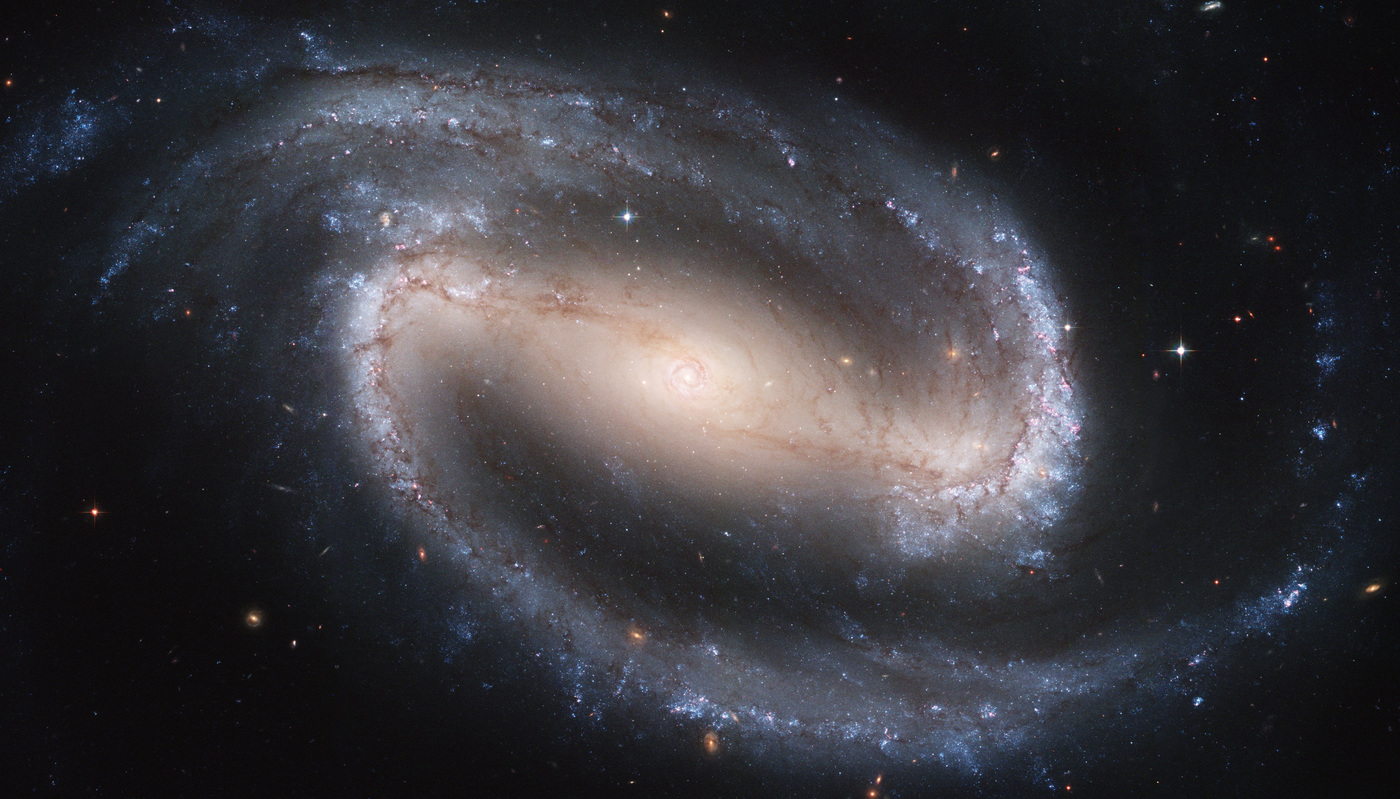
\includegraphics[width=0.99\columnwidth]{images/NGC1300.jpg}\caption{Example of a barred galaxy (``nebula''): NGC 1300}\end{figure}}
\vs p015 5:6 \ublistelem{4.}\bibnobreakspace \bibemph{Centrifugal Planetary Daughters.} Enormous suns, when in certain stages of development, and if their revolutionary rate greatly accelerates, begin to throw off large quantities of matter which may subsequently be assembled to form small worlds that continue to encircle the parent sun.
\vs p015 5:7 \ublistelem{5.}\bibnobreakspace \bibemph{Gravity\hyp{}deficiency Spheres.} There is a critical limit to the size of individual stars. When a sun reaches this limit, unless it slows down in revolutionary rate, it is doomed to split; sun fission occurs, and a new double star of this variety is born. Numerous small planets may be subsequently formed as a by\hyp{}product of this gigantic disruption.
\vs p015 5:8 \ublistelem{6.}\bibnobreakspace \bibemph{Contractural Stars.} In the smaller systems the largest outer planet sometimes draws to itself its neighbouring worlds, while those planets near the sun begin their terminal plunge. With your solar system, such an end would mean that the four inner planets would be claimed by the sun, while the major planet, Jupiter, would be greatly enlarged by capturing the remaining worlds. Such an end of a solar system would result in the production of two adjacent but unequal suns, one type of double star formation. Such catastrophes are infrequent except out on the fringe of the superuniverse starry aggregations.
\vs p015 5:9 \ublistelem{7.}\bibnobreakspace \bibemph{Cumulative Spheres.} From the vast quantity of matter circulating in space, small planets may slowly accumulate. They grow by meteoric accretion and by minor collisions. In certain sectors of space, conditions favour such forms of planetary birth. Many an inhabited world has had such an origin.
\vs p015 5:10 Some of the dense dark islands are the direct result of the accretions of transmuting energy in space. Another group of these dark islands have come into being by the accumulation of enormous quantities of cold matter, mere fragments and meteors, circulating through space. Such aggregations of matter have never been hot and, except for density, are in composition very similar to Urantia.
\vs p015 5:11 \ublistelem{8.}\bibnobreakspace \bibemph{Burned\hyp{}out Suns.} Some of the dark islands of space are burned\hyp{}out isolated suns, all available space\hyp{}energy having been emitted. The organized units of matter approximate full condensation, virtual complete consolidation; and it requires ages upon ages for such enormous masses of highly condensed matter to be recharged in the circuits of space and thus to be prepared for new cycles of universe function following a collision or some equally revivifying cosmic happening.
\vs p015 5:12 \ublistelem{9.}\bibnobreakspace \bibemph{Collisional Spheres.} In those regions of thicker clustering, collisions are not uncommon. Such an astronomic readjustment is accompanied by tremendous energy changes and matter transmutations. Collisions involving dead suns are peculiarly influential in creating widespread energy fluctuations. Collisional debris often constitutes the material nucleuses for the subsequent formation of planetary bodies adapted to mortal habitation.
\vs p015 5:13 \ublistelem{10.}\bibnobreakspace \bibemph{Architectural Worlds.} These are the worlds which are built according to plans and specifications for some special purpose, such as Salvington, the headquarters of your local universe, and Uversa, the seat of government of our superuniverse.
\vs p015 5:14 \pc There are numerous other techniques for evolving suns and segregating planets, but the foregoing procedures suggest the methods whereby the vast majority of stellar systems and planetary families are brought into existence. To undertake to describe all the various techniques involved in stellar metamorphosis and planetary evolution would require the narration of almost 100 different modes of sun formation and planetary origin. As your star students scan the heavens, they will observe phenomena indicative of all these modes of stellar evolution, but they will seldom detect evidence of the formation of those small, nonluminous collections of matter which serve as inhabited planets, the most important of the vast material creations.
\usection{The Spheres of Space}
\vs p015 6:1 Irrespective of origin, the various spheres of space are classifiable into the following major divisions:
\vs p015 6:2 \ublistelem{1.}\bibnobreakspace The suns --- the stars of space.
\vs p015 6:3 \ublistelem{2.}\bibnobreakspace The dark islands of space.
\vs p015 6:4 \ublistelem{3.}\bibnobreakspace Minor space bodies --- comets, meteors, and planetesimals.
\vs p015 6:5 \ublistelem{4.}\bibnobreakspace The planets, including the inhabited worlds.
\vs p015 6:6 \ublistelem{5.}\bibnobreakspace Architectural spheres --- worlds made to order.
\vs p015 6:7 \pc With the exception of the architectural spheres, all space bodies have had an evolutionary origin, evolutionary in the sense that they have not been brought into being by fiat of Deity, evolutionary in the sense that the creative acts of God have unfolded by a time\hyp{}space technique through the operation of many of the created and eventuated intelligences of Deity.
\vs p015 6:8 \pc \bibemph{The Suns.} These are the stars of space in all their various stages of existence. Some are solitary evolving space systems; others are double stars, contracting or disappearing planetary systems. The stars of space exist in no less than a thousand different states and stages. You are familiar with suns that emit light accompanied by heat; but there are also suns which shine without heat.
\vs p015 6:9 The trillions upon trillions of years that an ordinary sun will continue to give out heat and light well illustrates the vast store of energy which each unit of matter contains. The actual energy stored in these invisible particles of physical matter is well\hyp{}nigh unimaginable. And this energy becomes almost wholly available as light when subjected to the tremendous heat pressure and the associated energy activities which prevail in the interior of the blazing suns. Still other conditions enable these suns to transform and send forth much of the energy of space which comes their way in the established space circuits. Many phases of physical energy and all forms of matter are attracted to, and subsequently distributed by, the solar dynamos. In this way the suns serve as local accelerators of energy circulation, acting as automatic power\hyp{}control stations.
\vs p015 6:10 The superuniverse of Orvonton is illuminated and warmed by more than ten trillion blazing suns. These suns are the stars of your observable astronomic system. More than two trillion are too distant and too small ever to be seen from Urantia. But in the master universe there are as many suns as there are glasses of water in the oceans of your world\fnst{Assuming the present value of the volume of the oceans (together with their seas) to be $1.5 \times 10^{18}\,m^3$ and a standard 250\,ml glass of water we obtain the required total number of stars: $6\times 10^{21}$.}.
\vs p015 6:11 \pc \bibemph{The Dark Islands of Space.} These are the dead suns and other large aggregations of matter devoid of light and heat. The dark islands are sometimes enormous in mass and exert a powerful influence in universe equilibrium and energy manipulation. The density of some of these large masses is well\hyp{}nigh unbelievable. And this great concentration of mass enables these dark islands to function as powerful balance wheels, holding large neighbouring systems in effective leash. They hold the gravity balance of power in many constellations; many physical systems which would otherwise speedily dive to destruction in near\hyp{}by suns are held securely in the gravity grasp of these guardian dark islands. It is because of this function that we can locate them accurately. We have measured the gravity pull of the luminous bodies, and we can therefore calculate the exact size and location of the dark islands of space which so effectively function to hold a given system steady in its course.
\vs p015 6:12 \pc \bibemph{Minor Space Bodies.} The meteors and other small particles of matter circulating and evolving in space constitute an enormous aggregate of energy and material substance.
\vs p015 6:13 Many comets are unestablished wild offspring of the solar mother wheels, which are being gradually brought under control of the central governing sun. Comets also have numerous other origins. A comet’s tail points away from the attracting body or sun because of the electrical reaction of its highly expanded gases and because of the actual pressure of light and other energies emanating from the sun. This phenomenon constitutes one of the positive proofs of the reality of light and its associated energies; it demonstrates that light has weight. Light is a real substance, not simply waves of hypothetical ether.
\vs p015 6:14 \pc \bibemph{The Planets.} These are the larger aggregations of matter which follow an orbit around a sun or some other space body; they range in size from planetesimals to enormous gaseous, liquid, or solid spheres. The cold worlds which have been built up by the assemblage of floating space material, when they happen to be in proper relation to a near\hyp{}by sun, are the more ideal planets to harbour intelligent inhabitants. The dead suns are not, as a rule, suited to life; they are usually too far away from a living, blazing sun, and further, they are altogether too massive; gravity is tremendous at the surface.
\vs p015 6:15 In your superuniverse not one cool planet in 40 is habitable by beings of your order. And, of course, the superheated suns and the frigid outlying worlds are unfit to harbour higher life. In your solar system only three planets\fnst{The other two being Mars and Venus, according to A.S.\,Eddington, ``The Nature of the Physical World'', p.\,170, 1929.} are at present suited to harbour life. Urantia, in size, density, and location, is in many respects ideal for human habitation.
\vs p015 6:16 The laws of physical\hyp{}energy behaviour are basically universal, but local influences have much to do with the physical conditions which prevail on individual planets and in local systems. An almost endless variety of creature life and other living manifestations characterizes the countless worlds of space. There are, however, certain points of similarity in a group of worlds associated in a given system, while there also is a universe pattern of intelligent life. There are physical relationships among those planetary systems which belong to the same physical circuit, and which closely follow each other in the endless swing around the circle of universes.
\usection{The Architectural Spheres}
\vs p015 7:1 While each superuniverse government presides near the centre of the evolutionary universes of its space segment, it occupies a world made to order and is peopled by accredited personalities. These headquarters worlds are architectural spheres, space bodies specifically constructed for their special purpose. While sharing the light of near\hyp{}by suns, these spheres are independently lighted and heated. Each has a sun which gives forth light without heat, like the satellites of Paradise, while each is supplied with heat by the circulation of certain energy currents near the surface of the sphere. These headquarters worlds belong to one of the greater systems situated near the astronomical centre of their respective superuniverses.
\vs p015 7:2 \pc Time is standardized on the headquarters of the superuniverses. The standard day of the superuniverse of Orvonton is equal to almost 30 days of Urantia time, and the Orvonton year equals 100 standard days. This Uversa year is standard in the 7\ts{th} superuniverse, and it is 22 minutes short of 3,000 days of Urantia time, about 8.2 of your years.
\vs p015 7:3 \pc The headquarters worlds of the 7 superuniverses partake of the nature and grandeur of Paradise, their central pattern of perfection. In reality, all headquarters worlds are paradisiacal. They are indeed heavenly abodes, and they increase in material size, morontia beauty, and spirit glory from Jerusem to the central Isle. And all the satellites of these headquarters worlds are also architectural spheres.
\vs p015 7:4 The various headquarters worlds are provided with every phase of material and spiritual creation. All kinds of material, morontial, and spiritual beings are at home on these rendezvous worlds of the universes. As mortal creatures ascend the universe, passing from the material to the spiritual realms, they never lose their appreciation for, and enjoyment of, their former levels of existence.
\vs p015 7:5 \pc \bibemph{Jerusem,} the headquarters of your local system of Satania, has its 7 worlds of transition culture, each of which is encircled by 7 satellites, among which are the 7 mansion worlds of morontia detention, man’s first postmortal residence. As the term heaven has been used on Urantia, it has sometimes meant these 7 mansion worlds, the first mansion world being denominated the 1\ts{st} heaven, and so on to the 7\ts{th}.
\vs p015 7:6 \pc \bibemph{Edentia,} the headquarters of your constellation of Norlatiadek, has its 70 satellites of socializing culture and training, on which ascenders sojourn upon the completion of the Jerusem regime of personality mobilization, unification, and realization.
\vs p015 7:7 \pc \bibemph{Salvington,} the capital of Nebadon, your local universe, is surrounded by 10 university clusters of 49 spheres each. Hereon is man spiritualized following his constellation socialization.
\vs p015 7:8 \pc \bibemph{Uminor the third,} the headquarters of your minor sector, Ensa, is surrounded by the 7 spheres of the higher physical studies of the ascendant life.
\vs p015 7:9 \pc \bibemph{Umajor the fifth,} the headquarters of your major sector, Splandon, is surrounded by the 70 spheres of the advancing intellectual training of the superuniverse.
\vs p015 7:10 \pc \bibemph{Uversa,} the headquarters of Orvonton, your superuniverse, is immediately surrounded by the 7 higher universities of advanced spiritual training for ascending will creatures. Each of these 7 clusters of wonder spheres consists of 70 specialized worlds containing thousands upon thousands of replete institutions and organizations devoted to universe training and spirit culture wherein the pilgrims of time are re\hyp{}educated and re\hyp{}examined preparatory to their long flight to Havona. The arriving pilgrims of time are always received on these associated worlds, but the departing graduates are always dispatched for Havona direct from the shores of Uversa.
\vs p015 7:11 Uversa is the spiritual and administrative headquarters for approximately one trillion inhabited or inhabitable worlds. The glory, grandeur, and perfection of the Orvonton capital surpass any of the wonders of the time\hyp{}space creations.
\vs p015 7:12 \pc If all the projected local universes and their component parts were established, there would be slightly less than 500 billion\fnst{The exact number is: $7\times(1 + 7\times 70 + 10\times(70+1) + 1000\times(7+1) + 100000\times 647591) = 453,313,764,407$.} architectural worlds in the 7 superuniverses.
\usection{Energy Control and Regulation}
\vs p015 8:1 The headquarters spheres of the superuniverses are so constructed that they are able to function as efficient power\hyp{}energy regulators for their various sectors, serving as focal points for the directionization of energy to their component local universes. They exert a powerful influence over the balance and control of the physical energies circulating through organized space.
\vs p015 8:2 Further regulative functions are performed by the superuniverse power centres and physical controllers, living and semiliving intelligent entities constituted for this express purpose. These power centres and controllers are difficult of understanding; the lower orders are not volitional, they do not possess will, they do not choose, their functions are very intelligent but apparently automatic and inherent in their highly specialized organization. The power centres and physical controllers of the superuniverses assume direction and partial control of the 30 energy systems which comprise the gravita domain. The physical\hyp{}energy circuits administered by the power centres of Uversa require a little over 968,000,000 years to complete the encirclement of the superuniverse.
\vs p015 8:3 \pc Evolving energy has substance; it has weight, although weight is always relative, depending on revolutionary velocity, mass, and antigravity. Mass in matter tends to retard velocity in energy\fnst{Indeed, this is clear from the geometric nature of proper mass as the momentum $p_5 = m$ conjugated to the proper time $x^5 = \tau$, cf. the note on \bibref[23:3.2]{p023 3:2}.}; and the anywhere\hyp{}present velocity of energy represents: the initial endowment of velocity, minus retardation by mass encountered in transit, plus the regulatory function of the living energy controllers of the superuniverse and the physical influence of near\hyp{}by highly heated or heavily charged bodies.
\vs p015 8:4 The universal plan for the maintenance of equilibrium between matter and energy necessitates the everlasting making and unmaking of the lesser material units. The Universe Power Directors have the ability to condense and detain, or to expand and liberate, varying quantities of energy.
\vs p015 8:5 Given a sufficient duration of retarding influence, gravity would eventually convert all energy into matter were it not for two factors: First, because of the antigravity influences of the energy controllers, and second, because organized matter tends to disintegrate under certain conditions found in very hot stars and under certain peculiar conditions in space near highly energized cold bodies of condensed matter.
\vs p015 8:6 When mass becomes overaggregated and threatens to unbalance energy, to deplete the physical power circuits, the physical controllers intervene unless gravity’s own further tendency to overmaterialize energy is defeated by the occurrence of a collision among the dead giants of space, thus in an instant completely dissipating the cumulative collections of gravity. In these collisional episodes enormous masses of matter are suddenly converted into the rarest form of energy, and the struggle for universal equilibrium is begun anew. Eventually the larger physical systems become stabilized, become physically settled, and are swung into the balanced and established circuits of the superuniverses. Subsequent to this event no more collisions or other devastating catastrophes will occur in such established systems.
\vs p015 8:7 During the times of plus energy there are power disturbances and heat fluctuations accompanied by electrical manifestations. During times of minus energy there are increased tendencies for matter to aggregate, condense, and to get out of control in the more delicately balanced circuits, with resultant tidal or collisional adjustments which quickly restore the balance between circulating energy and more literally stabilized matter. To forecast and otherwise to understand such likely behaviour of the blazing suns and the dark islands of space is one of the tasks of the celestial star observers.
\vs p015 8:8 We are able to recognize most of the laws governing universe equilibrium and to predict much pertaining to universe stability. Practically, our forecasts are reliable, but we are always confronted by certain forces which are not wholly amenable to the laws of energy control and matter behaviour known to us. The predictability of all physical phenomena becomes increasingly difficult as we proceed outward in the universes from Paradise. As we pass beyond the borders of the personal administration of the Paradise Rulers, we are confronted with increasing inability to reckon in accordance with the standards established and the experience acquired in connection with observations having exclusively to do with the physical phenomena of the near\hyp{}by astronomic systems. Even in the realms of the seven superuniverses we are living in the midst of force actions and energy reactions which pervade all our domains and extend in unified equilibrium on through all regions of outer space.
\vs p015 8:9 The farther out we go, the more certainly we encounter those variational and unpredictable phenomena which are so unerringly characteristic of the unfathomable presence\hyp{}performances of the Absolutes and the experiential Deities. And these phenomena must be indicative of some universal overcontrol of all things.
\vs p015 8:10 The superuniverse of Orvonton is apparently now running down; the outer universes seem to be winding up for unparalleled future activities; the central Havona universe is eternally stabilized. Gravity and absence of heat (cold) organize and hold matter together; heat and antigravity disrupt matter and dissipate energy. The living power directors and force organizers are the secret of the special control and intelligent direction of the endless metamorphoses of universe making, unmaking, and remaking. Nebulae may disperse, suns burn out, systems vanish, and planets perish, but the universes do not run down.
\usection{Circuits of the Superuniverses}
\vs p015 9:1 The universal circuits of Paradise do actually pervade the realms of the seven superuniverses. These presence circuits are: the personality gravity of the Universal Father, the spiritual gravity of the Eternal Son, the mind gravity of the Conjoint Actor, and the material gravity of the eternal Isle.
\vs p015 9:2 In addition to the universal Paradise circuits and in addition to the presence\hyp{}performances of the Absolutes and the experiential Deities, there function within the superuniverse space level only two energy\hyp{}circuit divisions or power segregations: the superuniverse circuits and the local universe circuits.
\vs p015 9:3 \pc \bibemph{The Superuniverse Circuits:}
\vs p015 9:4 \ublistelem{1.}\bibnobreakspace The unifying intelligence circuit of one of the Seven Master Spirits of Paradise. Such a cosmic\hyp{}mind circuit is limited to a single superuniverse.
\vs p015 9:5 \ublistelem{2.}\bibnobreakspace The reflective\hyp{}service circuit of the seven Reflective Spirits in each superuniverse.
\vs p015 9:6 \ublistelem{3.}\bibnobreakspace The secret circuits of the Mystery Monitors, in some manner interassociated and routed by Divinington to the Universal Father on Paradise.
\vs p015 9:7 \ublistelem{4.}\bibnobreakspace The circuit of the intercommunion of the Eternal Son with his Paradise Sons.
\vs p015 9:8 \ublistelem{5.}\bibnobreakspace The flash presence of the Infinite Spirit.
\vs p015 9:9 \ublistelem{6.}\bibnobreakspace The broadcasts of Paradise, the space reports of Havona.
\vs p015 9:10 \ublistelem{7.}\bibnobreakspace The energy circuits of the power centres and the physical controllers.
\vs p015 9:11 \pc \bibemph{The Local Universe Circuits:}
\vs p015 9:12 \ublistelem{1.}\bibnobreakspace The bestowal spirit of the Paradise Sons, the Comforter of the bestowal worlds. The Spirit of Truth, the spirit of Michael on Urantia.
\vs p015 9:13 \ublistelem{2.}\bibnobreakspace The circuit of the Divine Ministers, the local universe Mother Spirits, the Holy Spirit of your world.
\vs p015 9:14 \ublistelem{3.}\bibnobreakspace The intelligence\hyp{}ministry circuit of a local universe, including the diversely functioning presence of the adjutant mind\hyp{}spirits.
\vs p015 9:15 \pc When there develops such a spiritual harmony in a local universe that its individual and combined circuits become indistinguishable from those of the superuniverse, when such identity of function and oneness of ministry actually prevail, then does the local universe immediately swing into the settled circuits of light and life, becoming at once eligible for admission into the spiritual confederation of the perfected union of the supercreation. The requisites for admission to the councils of the Ancients of Days, membership in the superuniverse confederation, are:
\vs p015 9:16 \ublistelem{1.}\bibnobreakspace \bibemph{Physical Stability.} The stars and planets of a local universe must be in equilibrium; the periods of immediate stellar metamorphosis must be over. The universe must be proceeding on a clear track; its orbit must be safely and finally settled.
\vs p015 9:17 \ublistelem{2.}\bibnobreakspace \bibemph{Spiritual Loyalty.} There must exist a state of universal recognition of, and loyalty to, the Sovereign Son of God who presides over the affairs of such a local universe. There must have come into being a state of harmonious co\hyp{}operation between the individual planets, systems, and constellations of the entire local universe.
\vs p015 9:18 \pc Your local universe is not even reckoned as belonging to the settled physical order of the superuniverse, much less as holding membership in the recognized spiritual family of the supergovernment. Although Nebadon does not yet have representation on Uversa, we of the superuniverse government are dispatched to its worlds on special missions from time to time, even as I have come to Urantia directly from Uversa. We lend every possible assistance to your directors and rulers in the solution of their difficult problems; we are desirous of seeing your universe qualified for full admission into the associated creations of the superuniverse family.
\usection{Rulers of the Superuniverses}
\vs p015 10:1 The headquarters of the superuniverses are the seats of the high spiritual government of the time\hyp{}space domains. The executive branch of the supergovernment, taking origin in the Councils of the Trinity, is immediately directed by one of the Seven Master Spirits of supreme supervision, beings who sit upon seats of Paradise authority and administer the superuniverses through the Seven Supreme Executives stationed on the seven special worlds of the Infinite Spirit, the outermost satellites of Paradise.
\vs p015 10:2 The superuniverse headquarters are the abiding places of the Reflective Spirits and the Reflective Image Aids. From this midway position these marvellous beings conduct their tremendous reflectivity operations, thus ministering to the central universe above and to the local universes below.
\vs p015 10:3 \pc Each superuniverse is presided over by three Ancients of Days, the joint chief executives of the supergovernment. In its executive branch the personnel of the superuniverse government consists of seven different groups:
\vs p015 10:4 \ublistelem{1.}\bibnobreakspace Ancients of Days.
\vs p015 10:5 \ublistelem{2.}\bibnobreakspace Perfectors of Wisdom.
\vs p015 10:6 \ublistelem{3.}\bibnobreakspace Divine Counsellors.
\vs p015 10:7 \ublistelem{4.}\bibnobreakspace Universal Censors.
\vs p015 10:8 \ublistelem{5.}\bibnobreakspace Mighty Messengers.
\vs p015 10:9 \ublistelem{6.}\bibnobreakspace Those High in Authority.
\vs p015 10:10 \ublistelem{7.}\bibnobreakspace Those without Name and Number.
\vs p015 10:11 \pc The three Ancients of Days are immediately assisted by a corps of one billion Perfectors of Wisdom, with whom are associated three billion Divine Counsellors. One billion Universal Censors are attached to each superuniverse administration. These three groups are Co\hyp{}ordinate Trinity Personalities, taking origin directly and divinely in the Paradise Trinity.
\vs p015 10:12 The remaining three orders, Mighty Messengers, Those High in Authority, and Those without Name and Number, are glorified ascendant mortals. The first of these orders came up through the ascendant regime and passed through Havona in the days of Grandfanda. Having attained Paradise, they were mustered into the Corps of the Finality, embraced by the Paradise Trinity, and subsequently assigned to the supernal service of the Ancients of Days. As a class, these three orders are known as Trinitized Sons of Attainment, being of dual origin but now of Trinity service. Thus was the executive branch of the superuniverse government enlarged to include the glorified and perfected children of the evolutionary worlds.
\vs p015 10:13 The co\hyp{}ordinate council of the superuniverse is composed of the seven executive groups previously named and the following sector rulers and other regional overseers:
\vs p015 10:14 \ublistelem{1.}\bibnobreakspace Perfections of Days --- the rulers of the superuniverse major sectors.
\vs p015 10:15 \ublistelem{2.}\bibnobreakspace Recents of Days --- the directors of the superuniverse minor sectors.
\vs p015 10:16 \ublistelem{3.}\bibnobreakspace Unions of Days --- the Paradise advisers to the rulers of the local universes.
\vs p015 10:17 \ublistelem{4.}\bibnobreakspace Faithfuls of Days --- the Paradise counsellors to the Most High rulers of the constellation governments.
\vs p015 10:18 \ublistelem{5.}\bibnobreakspace Trinity Teacher Sons who may chance to be on duty at superuniverse headquarters.
\vs p015 10:19 \ublistelem{6.}\bibnobreakspace Eternals of Days who may happen to be present at superuniverse headquarters.
\vs p015 10:20 \ublistelem{7.}\bibnobreakspace The seven Reflective Image Aids --- the spokesmen of the seven Reflective Spirits and through them representatives of the Seven Master Spirits of Paradise.
\vs p015 10:21 \pc The Reflective Image Aids also function as the representatives of numerous groups of beings who are influential in the superuniverse governments, but who are not, at present, for various reasons, fully active in their individual capacities. Embraced within this group are: the evolving superuniverse personality manifestation of the Supreme Being, the Unqualified Supervisors of the Supreme, the Qualified Vicegerents of the Ultimate, the unnamed liaison reflectivators of Majeston, and the superpersonal spirit representatives of the Eternal Son.
\vs p015 10:22 \pc At almost all times it is possible to find representatives of all groups of created beings on the headquarters worlds of the superuniverses. The routine ministering work of the superuniverses is performed by the mighty seconaphim and by other members of the vast family of the Infinite Spirit. In the work of these marvellous centres of superuniverse administration, control, ministry, and executive judgment, the intelligences of every sphere of universal life are mingled in effective service, wise administration, loving ministry, and just judgment.
\vs p015 10:23 The superuniverses do not maintain any sort of ambassadorial representation; they are completely isolated from each other. They know of mutual affairs only through the Paradise clearinghouse maintained by the Seven Master Spirits. Their rulers work in the councils of divine wisdom for the welfare of their own superuniverses regardless of what may be transpiring in other sections of the universal creation. This isolation of the superuniverses will persist until such time as their co\hyp{}ordination is achieved by the more complete factualization of the personality\hyp{}sovereignty of the evolving experiential Supreme Being.
\usection{The Deliberative Assembly}
\vs p015 11:1 It is on such worlds as Uversa that the beings representative of the autocracy of perfection and the democracy of evolution meet face to face. The executive branch of the supergovernment originates in the realms of perfection; the legislative branch springs from the flowering of the evolutionary universes.
\vs p015 11:2 The deliberative assembly of the superuniverse is confined to the headquarters world. This legislative or advisory council consists of seven houses, to each of which every local universe admitted to the superuniverse councils elects a native representative. These representatives are chosen by the high councils of such local universes from among the ascending\hyp{}pilgrim graduates of Orvonton who are tarrying on Uversa, accredited for transport to Havona. The average term of service is about 100 years of superuniverse standard time.
\vs p015 11:3 Never have I known of a disagreement between the Orvonton executives and the Uversa assembly. Never yet, in the history of our superuniverse, has the deliberative body ever passed a recommendation that the executive division of the supergovernment has even hesitated to carry out. There always has prevailed the most perfect harmony and working agreement, all of which testifies to the fact that evolutionary beings can really attain the heights of perfected wisdom which qualifies them to consort with the personalities of perfect origin and divine nature. The presence of the deliberative assemblies on the superuniverse headquarters reveals the wisdom, and foreshadows the ultimate triumph, of the whole vast evolutionary concept of the Universal Father and his Eternal Son.
\usection{The Supreme Tribunals}
\vs p015 12:1 When we speak of executive and deliberative branches of the Uversa government, you may, from the analogy of certain forms of Urantian civil government, reason that we must have a third or judicial branch, and we do; but it does not have a separate personnel. Our courts are constituted as follows: There presides, in accordance with the nature and gravity of the case, an Ancient of Days, a Perfector of Wisdom, or a Divine Counsellor. The evidence for or against an individual, a planet, system, constellation, or universe is presented and interpreted by the Censors. The defence of the children of time and the evolutionary planets is offered by the Mighty Messengers, the official observers of the superuniverse government to the local universes and systems. The attitude of the higher government is portrayed by Those High in Authority. And ordinarily the verdict is formulated by a varying\hyp{}sized commission consisting equally of Those without Name and Number and a group of understanding personalities chosen from the deliberative assembly.
\vs p015 12:2 The courts of the Ancients of Days are the high review tribunals for the spiritual adjudication of all component universes. The Sovereign Sons of the local universes are supreme in their own domains; they are subject to the supergovernment only in so far as they voluntarily submit matters for counsel or adjudication by the Ancients of Days except in matters involving the extinction of will creatures. Mandates of judgment originate in the local universes, but sentences involving the extinction of will creatures are always formulated on, and executed from, the headquarters of the superuniverse. The Sons of the local universes can decree the survival of mortal man, but only the Ancients of Days may sit in executive judgment on the issues of eternal life and death.
\vs p015 12:3 In all matters not requiring trial, the submission of evidence, the Ancients of Days or their associates render decisions, and these rulings are always unanimous. We are here dealing with the councils of perfection. There are no disagreements nor minority opinions in the decrees of these supreme and superlative tribunals.
\vs p015 12:4 With certain few exceptions the supergovernments exercise jurisdiction over all things and all beings in their respective domains. There is no appeal from the rulings and decisions of the superuniverse authorities since they represent the concurred opinions of the Ancients of Days and that Master Spirit who, from Paradise, presides over the destiny of the superuniverse concerned.
\usection{The Sector Governments}
\vs p015 13:1 A \bibemph{major sector} comprises about \bibfrac{1}{10}\ts{th} of a superuniverse and consists of 100 minor sectors, $10^4$ local universes, about $10^{11}$ inhabitable worlds. These major sectors are administered by three Perfections of Days, Supreme Trinity Personalities.
\vs p015 13:2 The courts of the Perfections of Days are constituted much as are those of the Ancients of Days except that they do not sit in spiritual judgment upon the realms. The work of these major sector governments has chiefly to do with the intellectual status of a far\hyp{}flung creation. The major sectors detain, adjudicate, dispense, and tabulate, for reporting to the courts of the Ancients of Days, all matters of superuniverse importance of a routine and administrative nature which are not immediately concerned with the spiritual administration of the realms or with the outworking of the mortal\hyp{}ascension plans of the Paradise Rulers. The personnel of a major sector government is no different from that of the superuniverse.
\vs p015 13:3 As the magnificent satellites of Uversa are concerned with your final spiritual preparation for Havona, so are the 70 satellites of Umajor the fifth devoted to your superuniverse intellectual training and development. From all Orvonton, here are gathered together the wise beings who labour untiringly to prepare the mortals of time for their further progress towards the career of eternity. Most of this training of ascending mortals is conducted on the 70 study worlds.
\vs p015 13:4 \pc The \bibemph{minor sector} governments are presided over by three Recents of Days. Their administration is concerned mainly with the physical control, unification, stabilization, and routine co\hyp{}ordination of the administration of the component local universes. Each minor sector embraces as many as 100 local universes, $10^4$ constellations, $10^6$ systems, or about $10^9$ inhabitable worlds.
\vs p015 13:5 Minor sector headquarters worlds are the grand rendezvous of the Master Physical Controllers. These headquarters worlds are surrounded by the seven instruction spheres which constitute the entrance schools of the superuniverse and are the centres of training for physical and administrative knowledge concerning the universe of universes.
\vs p015 13:6 The administrators of the minor sector governments are under the immediate jurisdiction of the major sector rulers. The Recents of Days receive all reports of observations and co\hyp{}ordinate all recommendations which come up to a superuniverse from the Unions of Days who are stationed as Trinity observers and advisers on the headquarters spheres of the local universes and from the Faithfuls of Days who are similarly attached to the councils of the Most Highs at the headquarters of the constellations. All such reports are transmitted to the Perfections of Days on the major sectors, subsequently to be passed on to the courts of the Ancients of Days. Thus the Trinity regime extends from the constellations of the local universes up to the headquarters of the superuniverse. The local system headquarters do not have Trinity representatives.
\usection{Purposes of the Seven Superuniverses}
\vs p015 14:1 There are seven major purposes which are being unfolded in the evolution of the seven superuniverses. Each major purpose in superuniverse evolution will find fullest expression in only one of the seven superuniverses, and therefore does each superuniverse have a special function and a unique nature.
\vs p015 14:2 Orvonton, the seventh superuniverse, the one to which your local universe belongs, is known chiefly because of its tremendous and lavish bestowal of merciful ministry to the mortals of the realms. It is renowned for the manner in which justice prevails as tempered by mercy and power rules as conditioned by patience, while the sacrifices of time are freely made to secure the stabilization of eternity. Orvonton is a universe demonstration of love and mercy.
\vs p015 14:3 It is, however, very difficult to describe our conception of the true nature of the evolutionary purpose which is unfolding in Orvonton, but it may be suggested by saying that in this supercreation we feel that the six unique purposes of cosmic evolution as manifested in the six associated supercreations are here being interassociated into a meaning\hyp{}of\hyp{}the\hyp{}whole; and it is for this reason that we have sometimes conjectured that the evolved and finished personalization of God the Supreme will in the remote future and from Uversa rule the perfected seven superuniverses in all the experiential majesty of his then attained almighty sovereign power.
\vs p015 14:4 As Orvonton is unique in nature and individual in destiny, so also is each of its six associated superuniverses. A great deal that is going on in Orvonton is not, however, revealed to you, and of these unrevealed features of Orvonton life, many are to find most complete expression in some other superuniverse. The seven purposes of superuniverse evolution are operative throughout all seven superuniverses, but each supercreation will give fullest expression to only one of these purposes. To understand more about these superuniverse purposes, much that you do not understand would have to be revealed, and even then you would comprehend but little. This entire narrative presents only a fleeting glimpse of the immense creation of which your world and local system are a part.
\vs p015 14:5 \pc Your world is called Urantia, and it is number 606 in the planetary group, or system, of Satania. This system has at present 619 inhabited worlds, and more than 200 additional planets are evolving favourably toward becoming inhabited worlds at some future time.
\vs p015 14:6 Satania has a headquarters world called Jerusem, and it is system number 24 in the constellation of Norlatiadek. Your constellation, Norlatiadek, consists of 100 local systems and has a headquarters world called Edentia. Norlatiadek is number 70 in the universe of Nebadon. The local universe of Nebadon consists of 100 constellations and has a capital known as Salvington. The universe of Nebadon is number 84 in the minor sector of Ensa.
\vs p015 14:7 The minor sector of Ensa consists of 100 local universes and has a capital called Uminor the 3\ts{rd}. This minor sector is number 3 in the major sector of Splandon. Splandon consists of 100 minor sectors and has a headquarters world called Umajor the 5\ts{th}. It is the 5\ts{th} major sector of the superuniverse of Orvonton, the 7\ts{th} segment of the grand universe. Thus you can locate your planet in the scheme of the organization and administration of the universe of universes.
\vs p015 14:8 The grand universe number of your world, Urantia, is 5,342,482,337,666\fnst{How are the 7 celestial coordinates of our planet just given (7, 5, 3, 84, 70, 24, 606) encoded in the registry number? It is possible that the \bibemph{decimal} status is included as well and, together with the planet's number 606, it is represented in the final digits 666, see the note on \bibref[58:1.1]{p058 1:1}.}. That is the registry number on Uversa and on Paradise, your number in the catalogue of the inhabited worlds. I know the physical\hyp{}sphere registry number, but it is of such an extraordinary size that it is of little practical significance to the mortal mind.
\vs p015 14:9 \pc Your planet is a member of an enormous cosmos; you belong to a well\hyp{}nigh infinite family of worlds, but your sphere is just as precisely administered and just as lovingly fostered as if it were the only inhabited world in all existence.
\vsetoff
\vs p015 14:10 [Presented by a Universal Censor hailing from Uversa.]
\quizlink
\begin{thebibliography}{100}
\bibitem{Eddington1}
Sir Arthur Stanley Eddington.
{<<The Nature of the Physical World>>.}
{\em Cambridge, England}, 1929.
\bibitem{Baker1}
Robert H. Baker, Ph.D.
{<<The Universe Unfolding: A Story of Man's Increasing Comprehension of the Universe Around Him.>>}
{\em Baltimore: The Williams \&\ Wilkins Company}, 1932.
\bibitem{Barnes1}
Ernest William Barnes.
{<<Scientific Theory and Religion: The World described by Science and its Spiritual interpretation>>.}
{\em Cambridge: At the University Press}, 1933.
\bibitem{Swann1}
W.F.G.~Swann.
{``The Architecture of the Universe''}
{\em New York: The Macmillan Company}, 1934.
\end{thebibliography}
